\documentclass[a4paper,12pt]{article}
\usepackage{amsmath,amsfonts,amsthm,amssymb, mathtools,steinmetz, gensymb, siunitx}	% LOADS USEFUL MATH STUFF
\usepackage{xcolor,graphicx}
\usepackage[a4paper]{geometry} 				% ADJUSTS PAGE
\usepackage{setspace}
\usepackage{physics}
\usepackage{caption}
\usepackage{tikz}
\usepackage{pgf,tikz,pgfplots}
\usepackage{mathrsfs}
\usepackage{amsbsy}
\usepackage{fancyhdr}
\usepackage{float}
\usepackage{array}
\usepackage{booktabs}
\usepackage{newpxtext}
\usepackage{unicode-math}
\usepackage{braket}
\usepackage{tensor}
\setmathfont{Libertinus Math}

\usetikzlibrary{decorations.pathreplacing,decorations.markings}
\usepgfplotslibrary{fillbetween}

\newgeometry{left=1cm,top = 2.5cm, bottom = 1.75cm, right = 1cm}

\newcommand{\defeq}{:=}
\newcommand\block[1]{\hspace*{#1}}
\newcommand{\rpm}{\sbox0{$1$}\sbox2{$\scriptstyle\pm$}
	  \raise\dimexpr(\ht0-\ht2)/2\relax\box2 }
\newcommand{\af}{\pmb{\hat a_1}}
\newcommand{\as}{\pmb{\hat a_2}}
\newcommand{\at}{\pmb{\hat a_3}}
\newcommand\uv[1]{\pmb{\hat {#1}}}
\newcommand\vect[1]{\pmb{{#1}}}
\newcommand\dprod{\pmb{\cdot}}

\usepackage{tabstackengine}
\setstackEOL{;}% row separator
\setstackTAB{,}% column separator
\setstacktabbedgap{1ex}% inter-column gap
\setstackgap{L}{1.0\normalbaselineskip}% inter-row baselineskip
\newcommand\rbm[1]{\left(\Matrixstack{#1}\right)}
	  
\pgfplotsset{compat=newest}
\newlength{\QNo}
\settowidth{\QNo}{2.}

\newlength{\QLetter}
\settowidth{\QLetter}{(a)}

\pagestyle{fancy}
\rhead{Quantum mechanics Problem Set}
\lhead{J. L. Gouws}


\begin{document}
\fontencoding{T1}
\fontfamily{ppl}\selectfont
{\Large \textbf{Quantum mechanics Assignment 1}} \hfill {\Large \textbf{J L Gouws}}\\
\block{1.0cm} {\large \textbf{\today}} \hfill {\large \textbf{26634554}}\\
\thispagestyle{empty}
\fontencoding{T1}

1.
\begin{minipage}[t]{0.9\textwidth}
  \begin{align*}
    \left(\bra{\psi} + \alpha^* \bra{\phi}\right)\left(\alpha \ket{\phi} + \ket{\psi}\right) &= \bra{\psi}\left(\alpha \ket{\phi} + \ket{\psi}\right) + \alpha^* \bra{\phi}\left(\alpha \ket{\phi} + \ket{\psi}\right)\\
                                                                                             &= \alpha \braket{\psi|\phi} + \braket{\psi|\psi} + |\alpha|^2 \braket{\phi | \phi}+ \alpha^*\braket{\phi|\psi}\\
                                                                                             & \geq 0\\
  \end{align*}
  The above statement holds for all $\alpha$, and in particular $\alpha = i\frac{\braket{\psi|\phi}}{\braket{\phi | \phi}}$.
  If we substitute this choice of $\alpha$ into the inequality above, we get:
  \begin{align*}
    \Rightarrow & i \frac{|\braket{\psi|\phi}|^2}{\braket{\phi|\phi}} + \braket{\psi|\psi} - |\braket{\psi|\phi}|^2\frac{\braket{\phi | \phi}}{|\braket{\phi | \phi}|^2} - i \frac{|\braket{\phi|\psi}|^2}{\braket{\phi|\phi}} \geq 0\\
    \Rightarrow & \braket{\psi|\psi} - \frac{|\braket{\psi|\phi}|^2}{\braket{\phi | \phi}} \geq 0\\
    \Rightarrow & \braket{\psi|\psi} \braket{\phi | \phi} \geq |\braket{\psi|\phi}|^2\\
  \end{align*}
  Which is the required result. 
\end{minipage}

\iffalse
\begin{figure}
  \centering
  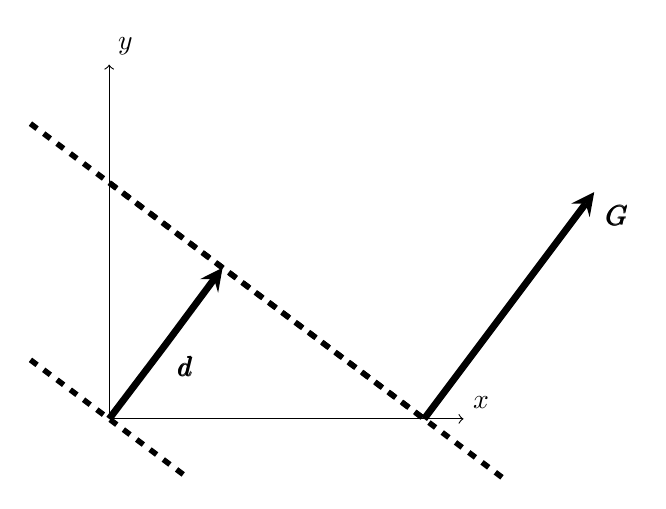
\begin{tikzpicture}
    \draw[->] (0, 0) -- (4.5, 0) node[anchor = south west] {$x$};
    \draw[->] (0, 0) -- (0, 4.5) node[anchor = south west] {$y$};
    \draw[dashed, line width = 2] (-1, 3.75) -- (5, -0.75);
    \draw[dashed, line width = 2] (-1, .75) -- (1, -0.75);
    \draw[dashed, line width = 2] (0, 3) -- (4, 0);
    \draw[->, line width = 2.5, >=stealth] (0, 0) --  (0.72, 0.95) node[anchor = north west] {$\pmb{d}$}-- (1.44, 1.92);
    \draw[->, line width = 2.5, >=stealth] (4, 0) -- (6.16, 2.88) node[anchor = north west] {$\pmb{G}$};
  \end{tikzpicture}
  \caption{The interplanar separation.}
  \label{fig:planeSep}
\end{figure}

\begin{figure}
  \centering
  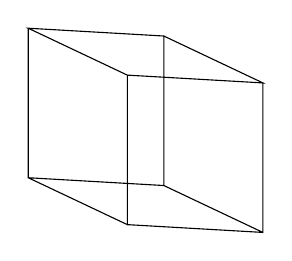
\begin{tikzpicture}
    \begin{axis}[
      axis x line=none,
      axis y line=none,
      axis z line=none,
      axis equal image,
%      view = {20}{30}
    ]
    \addplot3 [mark=none] coordinates 
    {
      (0, -1, 2)
      (3, 0, 2)
      (0, 1, 2)
      (-3, 0, 2)
      (0, -1, 2)
      (0, -1, -2)
      (3, 0, -2)
      (3, 0, 2)
      (3, 0, -2)
      (0, 1, -2)
      (0, 1, 2)
      (0, 1, -2)
      (-3, 0, -2)
      (-3, 0, 2)
      (-3, 0, -2)
      (0, -1, -2)
      (0, -1, 2)
      (0, -1, -2)
    };
    \end{axis}
  \end{tikzpicture}
  \caption{The first Brillouin zone of a hexagonal lattice}
  \label{fig:firsBrillouin}
\end{figure}
\fi

2.
\begin{minipage}[t]{0.9\textwidth}
  a).
  \begin{minipage}[t]{\textwidth}
    Let $\left(\begin{matrix} a & b \\ c & d\end{matrix}\right)$ be a general matrix over $\mathbb{C}$.\\
    Then we need to find $\alpha, \beta, \gamma, \delta \in \mathbb{C}$, such that:
    \begin{equation*}
      \left(\begin{matrix} a & b \\ c & d\end{matrix}\right) = \alpha \left(\begin{matrix}1 & 0 \\ 0 & 1\end{matrix}\right)
        + \beta \left(\begin{matrix}0 & 1 \\ 1 & 0\end{matrix}\right) + \gamma \left(\begin{matrix}0 & -i \\ i & 0\end{matrix}\right) + \delta\left(\begin{matrix}1 & 0 \\ 0 & -1\end{matrix}\right)
    \end{equation*}
    For this we have:
    \begin{align*}
      a &= \alpha + \delta\\
      b &= \beta + -i\gamma\\
      c &= \beta  + i\gamma\\
      d &= \alpha - \delta
    \end{align*}
    This system of equations is partially decoupled, and so is easily solved.
    \begin{align*}
      \alpha  &= \frac{a + d}{2}\\
      \beta &= \frac{b + c}{2}\\
      \gamma &= i\frac{b - c}{2}\\
      \delta &= \frac{a - d}{2} 
    \end{align*}
    Since $a, b, c, d$ are in $\mathbb{C}$ and $\mathbb{C}$ is a field, $\alpha, \beta, \gamma, \delta$ are definitely in $\mathbb{C}$ as required.
  \end{minipage}
\end{minipage}

\begin{minipage}[t]{\textwidth}
  b).
  \begin{minipage}[t]{\textwidth}
    $\trace\left({A^\dagger B}\right)$ is an inner product:
    First, $\left(A, B\right) = \trace\left(A^\dagger B\right)$, is indeed a map $\mathbb{C}^{2\times 2}\times \mathbb{C}^{2\times 2} \to \mathbb{C}$.\\
    Let:
    \begin{equation*}
      A = \rbm{a_{11}, a_{12}; a_{21}, a_{22}} \qquad \qquad B = \rbm{b_{11}, b_{12}; b_{21}, b_{22}} \qquad  \qquad C = \rbm{c_{11}, c_{12}; c_{21}, c_{22}}
    \end{equation*}
    Note:
    \begin{align*}
      \left( A, B \right) &= \trace\left\{\rbm{a_{11}^*, a_{21}^*; a_{12}^*, a_{22}^*} \rbm{b_{11}, b_{12}; b_{21}, b_{22}}\right\}\\
      & = \trace\left\{\rbm{a_{11}^*b_{11} + a_{21}^* b_{21}, a_{11}^*b_{12} + a_{21}^*b_{22}; a_{12}^*b_{11} + a_{22}^*b_{21}, a_{12}^*b_{12} + a_{22}^* b_{22}} \right\} \\
      &= a_{11}^*b_{11} + a_{21}^* b_{21} + a_{12}^*b_{12} + a_{22}^* b_{22}
    \end{align*}
    Similarly
    \begin{align*}
      \left(B, A \right) = b_{11}^*a_{11} + b_{21}^* a_{21} + b_{12}^*a_{12} + b_{22}^* a_{22}
    \end{align*}
    It is now clear that:
    \begin{equation*}
      \left( B, A \right)^* = \left(b_{11}^*a_{11} + b_{21}^* a_{21} + b_{12}^*a_{12} + b_{22}^* a_{22}\right)^* = a_{11}^*b_{11} + a_{21}^* b_{21} + a_{12}^*b_{12} + a_{22}^* b_{22} = \left( A, B\right)
    \end{equation*}
    As required, now moving onto linearity in the second argument:
    \begin{align*}
      \left(A , cB + dC \right) &= \trace\left\{A^\dagger\left(cB + dC\right)\right\}\\
                    &= \trace\left\{\rbm{a_{11}^*, a_{21}^*; a_{12}^*, a_{22}^*} \rbm{cb_{11} + dc_{11}, cb_{12} + d c_{12}; cb_{21}+ d c_{21}, cb_{22}+ d c_{22}}\right\}\\
                    &= a_{11}^*(cb_{11} + dc_{11}) + a_{21}^* (cb_{21} + dc_{21}) + a_{12}^*(cb_{12} + dc_{12}) + a_{22}^* (cb_{22}+ dc_{22})\\
                    &= c\left(a_{11}^*b_{11} + a_{21}^* b_{21} + a_{12}^*b_{12} + a_{22}^*b_{22} \right)+ d\left(a_{11}^*c_{11}  + a_{21}^* c_{21}  + a_{12}^*c_{12} + a_{22}^*c_{22}\right)\\
                    &= c\trace(A^\dagger B) + d\trace(A^\dagger C)\\
                    &= c\left(A, B\right) + d\left(A, C\right)
    \end{align*}
    Positive definiteness is shown by:
    \begin{align*}
      \left(A , A \right) &= a_{11}^*a_{11} + a_{12}^*a_{12} + a_{21}^*a_{21} + a_{22}^*a_{22}\\
                          &= |a_{11}|^2 + |a_{12}|^2 + |a_{21}|^2 + |a_{22}|^2\\
                          & \geq 0\\
    \end{align*}
    and since $|c| = 0 \Leftrightarrow c = 0$ for any $c \in \mathbb{C}$.
    We have form the above:
    \begin{align*}
      \left(A , A \right) = 0 \Leftrightarrow A = \rbm{0, 0; 0,0}
    \end{align*}
  \end{minipage}
\end{minipage}

3.
\begin{minipage}[t]{0.9\textwidth}
  \begin{minipage}[t]{\textwidth}
    Let the basis of our ket space be given by $\left\{\ket{a}\right\}$, that is the set of eigenkets of $A$.
    Now:
    \begin{equation*}
      A^n = A^n\sum_a \ket{a}\bra{a} = \sum_a A^n\ket{a}\bra{a} = \sum_a a^n\ket{a}\bra{a}
    \end{equation*}
    And similarly:
    \begin{equation*}
      A^m = \sum_a a^m\ket{a}\bra{a}
    \end{equation*}
    Thus
    \begin{align*}
      A^nA^m &= \left(\sum_a a^n\ket{a}\bra{a}\right)\left(\sum_{a'} a'^m\ket{a'}\bra{a'}\right)\\
             &= \sum_a \sum_{a'} a^na'^m\ket{a}\braket{a | 'a}\bra{a}\\
             &= \sum_a \sum_{a'} a^na'^m\ket{a}\tensor{\delta}{^a_{a'}}\bra{a}\\
             &= \sum_a a^na^m\ket{a}\bra{a}\\
             &= \sum_a a^{n + m}\ket{a}\bra{a}\\
             &\equiv A^{n + m}
    \end{align*}
  \end{minipage}
\end{minipage}

4.
\begin{minipage}[t]{0.9\textwidth}
  a).
  \begin{minipage}[t]{\textwidth}
    By definition:
    \begin{equation*}
      \trace{A} = \sum_i \braket{i|A|i}
    \end{equation*}
    Now:
    \begin{align*}
      \trace(AB) &= \sum_i \braket{i|AB|i}\\
                 &= \sum_i\sum_j \braket{i|A|j}\braket{j|B|i}\\
                 &= \sum_i\sum_j \braket{j|B|i}\braket{i|A|j}\\
                 &= \sum_j \braket{j|BA|j}\\
                 &= \trace(BA)
    \end{align*}

  \end{minipage}

  b).
  \begin{minipage}[t]{\textwidth}
    We have:
    \begin{align*}
      AB &= \sum_{i} AB\ket{i}\bra{i}\\
         &= \sum_{i}\sum_{j} A\ket{j} \bra{j}B\ket{i}\bra{i}\\
         &= \sum_{i}\sum_{j}\sum_{k} \ket{k} \bra{k}A\ket{j} \bra{j}B\ket{i}\bra{i}\\
         &= \sum_{i}\sum_{j}\sum_{k}  \bra{k}A\ket{j} \bra{j}B\ket{i} \ket{k}\bra{i}\\
    \end{align*}
    Now last expression above is just the sum of a number, $\braket{k|A|j}\braket{j|B|i}$, times by an operator and so:
    \begin{align*}
      (AB)^\dagger &= \sum_{i}\sum_{j}\sum_{k} \left(\bra{k}A\ket{j} \bra{j}B\ket{i} \ket{k}\bra{i}\right)^\dagger\\
                   &= \sum_{i}\sum_{j}\sum_{k} \left(\bra{k}A\ket{j} \bra{j}B\ket{i}\right)^* \ket{i}\bra{k}\\
                   &= \sum_{i}\sum_{j}\sum_{k} \bra{j}A^\dagger\ket{k} \bra{k}B^\dagger\ket{j} \ket{i}\bra{k}\\
                   &= \sum_{i}\sum_{j}\sum_{k} \bra{j}A^\dagger\ket{k} \bra{k}B^\dagger\ket{j} \ket{i}\bra{k}\\
    \end{align*}
  \end{minipage}
\end{minipage}
\end{document}
